\section{Трансверсали.}

\opri Пусть $2^{X}$ - булеан множества $X$, т.е. совокупность всех подмножеств множества $X$. Пусть $(X_1; \dots; X_n)$ - некоторая $n$-выборка из булеана. Вектор $(x_1; \dots; x_n)$, состоящий из элементов множества $X$, называется трансверсалью семейства $(X_1; \dots; X_n)$, если выполнены следующие отношения:

\begin{enumerate}
\item $x_i \in X_i$ ; $1 \leq i \leq n$;
\item $x_i \neq x_j$ ; $i \neq j$; $1 \leq i$, $j \leq n$.
\end{enumerate}

Иными словами имеем систему различных представителей семейства $(X_1; \dots; X_n)$ .\\
Обозначается $(x_1; \dots; x_n)$ тр. $(X_1; \dots; X_n)$

\thr \textbf{(Критерий Ф.Холла)}
Для того, чтобы семейство $(X_1; \dots; X_n)$ имело трансверсаль, необходимо и достаточно, чтобы $\forall$ k $\in \overline{1,n}$ и $\forall$ k-сочетания $i \leq j_1 \leq \dots \leq j_k \leq n$ выполнялось условие:

\begin{center}
$|X_{j_1} \cup \dots \cup X_{j_k}|\geq k$. (*)
\end{center}

\proof

\emph{Необходимость:}\\
Пусть $\exists (x_1; \dots; x_n)$ тр. $(X_1; \dots; X_n)$. Тогда $\forall k \in \overline{1,n}$ и $\forall$ набора $1 \leq j_1 \leq \dots \leq j_k\leq n$ имеем $x_{j_1} \in X_{j_1}, \dots, x_{j_k} \in X_{j_k}$ и $x_{j_s} \neq x_{j_t}$ при $j_t \neq j_s \Rightarrow |X_{j_1} \cup \dots \cup X_{j_k}| \geq k = |{x_1; \dots; x_k}|$.

\emph{Достаточность:}\\
Индукция по $n$. Пусть $n=1$ , тогда
$|X_1| \geq 1 \Rightarrow {x_1}$ тр $X_1$ .
Предположение индукции: $\forall n' < n$ из условия (*) $\Rightarrow \exists$ трансверсали для $n'$ множеств. 

Рассмотрим 2 случая:

а) Для всех $1 \leq k \leq n-1$ и $\forall j_1 < \dots < j_k \leq n$ верно $|X_{j_1} \cup \dots \cup X_{j_k}| \geq k+1$ (**)
При $k=1$ $|X_1| \geq 2 \Rightarrow \exists$ трансверсаль $x_1$ тр. $X$.

Рассмотрим семейство $(X_2'; \dots; X_n')$, где $X_i'=X_i \textbackslash \{x_i\}, 2 \leq i \leq n$.
Согласно (**) для этого семейства при $\forall 1 \leq k < n$ и $\forall 2 \leq j_1 < \dots < j_k \leq n$ имеем $|X_{j_1}' \cup \dots \cup X_{j_k}'| \geq k$ и по предположению индукции существует $(x_2; \dots; x_n)$ тр. $(X_2'; \dots; X_n')$, но тогда $(x_1, x_2, \dots, x_n)$ тр. $(X_1; \dots; X_n)$.

б) $\exists k$ и такое сочетание $1 \leq j_1 < \dots < j_k \leq n$, что $|X_{j_1} \cup \dots \cup X_{j_k}|=k$.

Т.к. можно перенумеровать подмножества, то не ограничивая общности считаем $|X_1 \cup \dots \cup X_k|=k$. По предположению индукции $\exists$ трансверсаль $(x_1; \dots; x_k)$ тр. $(X_1; \dots; X_k)$, т.к. $k<n$ и $\{x_1;\dots;x_k\}=|X_1 \cup \dots \cup X_k|$.

Рассмотрим семейство множеств $(X_{k+1}'; \dots; X_n')$, где $X_i'=X_i \textbackslash \{x_1;\dots;x_k\}, k+1 \leq i \leq n$. Для этого семейства верно условие (*), т.к. $\forall 1 \leq l \leq k$ и $\forall 1 \leq \nu_1 < \dots < \nu_l \leq n-k$ имеем $|X_{k+{\nu_1}}' \cup \dots \cup X_{k+{\nu_l}}' \cup X_1 \dots \cup X_k|-k\geq$
(Штрихи можно снять, т.к. $\{x_1; \dots; x_k\}$ и так содержится в $X_1 \cup \dots \cup X_k$).
$\geq k+l-k=1$, т.к. верно условие (*) для нештрихованных множеств. Таким образом $\exists  (x_{k+1}; \dots; x_n)$ тр. $(X_{k+1}'; \dots; X_n') \Rightarrow \exists (x_1; \dots; x_n)$ тр. $(X_1; \dots; X_n)$.\\

\examplei
\begin{enumerate}
    \item Представители различных классов эквивалентности.
    \item Остовное дерево графа. Его ребра - трансверсали множества рёбер графа.
\end{enumerate}

\opr Пусть $P=GF(q)$ - конечное поле из $q$ элементов, $q=p^d$, где $p \in \mathbb{P}$ (простое). Пусть $F(x)$ - реверсивный многочлен (т.е. $F(0) \neq 0 )$ над $P$. Найдутся $a \in P$ и $k \in \N : F(x)| x^k - a.$ Наименьшее $k$ с таким свойством назовём редуцированным периодом (Обозначение: $T_{red}(F)$). Элемент $a$ назовём мультипликатором многочлена $F(x)$. Обозначение $(Mult(F))$ - множество всех мультипликаторов.

Пусть $F(x)|x^t - b$, где $t = T_{red}(F)$.

\utv
\begin{enumerate}
\item $Mult(F) = <b>$;
\item $t \cdot |Mult(F)|=T_{red}(F)$;
\item  Если $f$ - примитивный, то $t= \frac{q^m - 1}{q-1}$, где $m=deg(f(x)), Mult(F)=P^*, b=F(0)$.
\end{enumerate}

Рассмотрим следующую модель ДСЧ (Датчик случайных чисел).\\

\begin{figure}[h!]
    \centering
    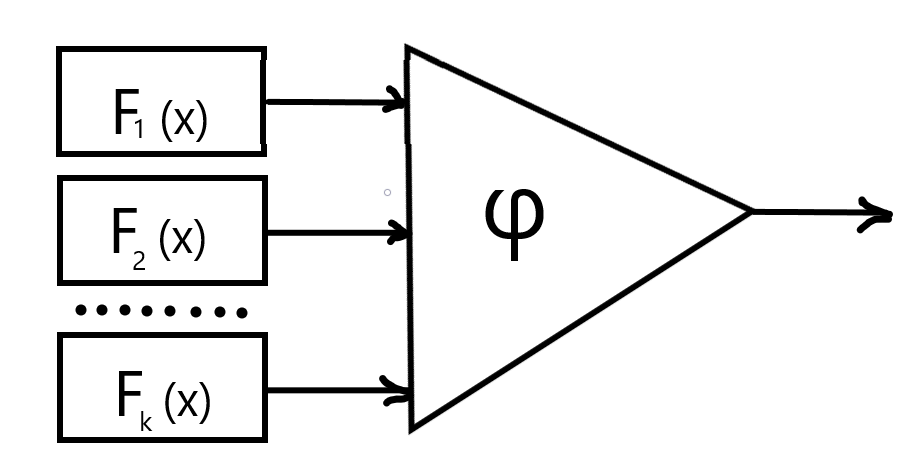
\includegraphics[scale=0.35]{DSC}
\end{figure}

Пусть $F_1, \dots, F_k$ - многочлены попарно взаимопростых степеней $m_1, \dots m_k$.

Тогда,
$$
T=[T(F_1), \dots, T(F_k)] = \frac{(q^{m_1} - 1) \cdot \ldots \cdot (q^{m_k} - 1)}{(q-1)^{k-1}}.
$$

$(q^{m_1} - 1) \cdot \dotsc \cdot (q^{m_k} - 1)$, каждый из них лежит на цикле длины $T$ и таких циклов $(q-1)^{k-1}$ . Будем считать, что начальное состояние $\vec{\alpha_0} = (u_1(0), \dots, u_1(m_1 - i),u_2(0),\dotsc, u_2(m_2-1), \dots, u_k(0), \dots, u_k(m_k-1))$ выбирается из множества $S$ всех состояний, тогда $\vec{\alpha_i}=(u_i(i), \dots, u_i(i+m_1-1), \dots, u_k(i), \dots, u_k(i+m_k-1) \in S$.
Последовательность $((\vec{\alpha_i})_{i=0}^{\infty})$ - чисто периодическая с периодом $T$.
Каждый вектор $\vec{\alpha} \in S$ запишем в виде $\vec{\alpha} = (\vec{\alpha}(1); \dots; \vec{\alpha}(k))$ , где $\vec{\alpha}(j) \in P^{m_j} \textbackslash \{\vec{0}\}$.

Зададим отношение $\sim : \forall \vec{\alpha}, \vec{\beta} \: \vec{\alpha}\sim\vec{\beta} \Leftrightarrow \exists c_1, \dots, c_k \in P^*|\vec{\alpha}(j) = c_j \vec{\beta}(j) \forall j \in \overline{1,k}$

Пусть $a_j$ - корень многочлена $F_j(x)$ в расширении $GF(q^{m_j})$ поля $P$, где $j \in \overline{1,k}$. Из пункта 3 утверждения следует, что $b_j = a_j \frac{q^{m_j}-1}{q-1} = a_j^{T_{red}(F_j)}, i \in \overline{1,k}$ , т.е. имеем мультипликатор многочлена $F_j(x)$ . Пусть $m=m_1; \dots; m_k$, положим $\forall \vec{\alpha}, \vec{\beta} \in S \: \vec{\alpha} \stackrel{red}{\sim} \vec{\beta} \Leftrightarrow \exists i \in \{0, \dots, q-2\} | \vec{\alpha}(j) = \vec{\beta}(j) * b^{m-i/n_j}, \forall j \in \overline{1,k}$ .

Для любого вектора $\exists$ ровно $q-1$ вектор, находящийся с ним в отношении $\stackrel{red}{\sim}$ .

\thr
Пусть $\vec{\gamma_1}, \vec{\gamma_2} \in S$, тогда

1) $\vec{\gamma_1} \sim \vec{\gamma_2}$

2) $\vec{\gamma_1} \bcancel{\stackrel{red}{\sim}} \vec{\gamma_2}$%ну не вот это отношение перечеркнутое типа, вы поняли?

Тогда $\vec{\gamma_1}$ и $\vec{\gamma_2}$ лежат на различных циклах. 